\chapter{Sequential Recommendations using Markov Chains}
\label{chapter:model_based}

Model-based mathematical methods for sequential recommender systems have been around for a very long time, even before neural networks became popular. They are often easy to understand and implement, and they produce state-of-the-art prediction results~\cite{zimdars2013using,hu2008collaborative}. As such, they are still the primary choice in many modern systems. The most popular model-based method for sequential recommender systems is Markov chains. In the following sections, we want to demonstrate how we can utilize Markov chains for sequential recommendations.

\section{Markov Chains}
\label{sec:markov_chains}

\begin{figure}[htbp]
\centering
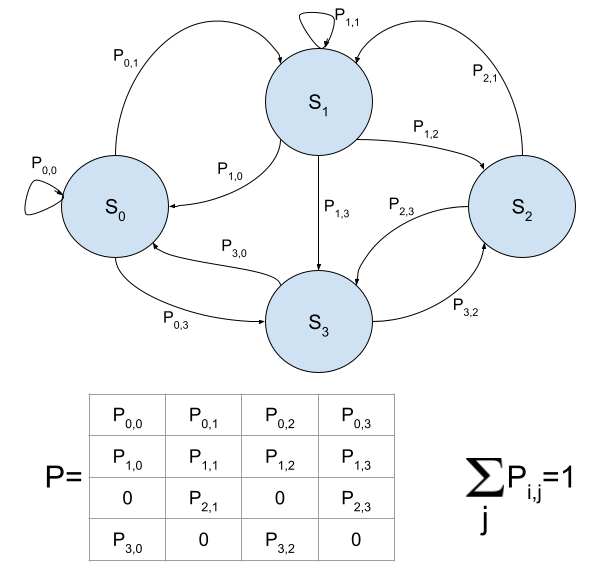
\includegraphics[width=0.7\textwidth]{images/diagrams/markov_chain.png}
\caption{The image shows a Markov chain with 4 states and the transition probabilities going from one state to another. In the transition matrix we can see the transition probabilities. The column number represents the current state and the row number the next state.}
\label{fig:markov_chains}
\end{figure}

Markov chains model processes that transition between different states $S=\{S_0, S_1, ..., S_n\}$ over time. Transitions between a state $S_i$ and $S_j$ are random but happen with the probability $P_{i,j}$. A process remains in the same state with probability $P_{i,i}$. We typically represent transition probabilities in matrix form. To get a transition probability, we can look at the rows and columns. The column number represents the current state and the row number the next state. Each row sums up to 1 because the process will transition or stay in the same state, with 100\% probability. Illustrated in Figure~\ref{fig:markov_chains} are a sample Markov chain and the associated transition matrix. Transition probabilities only depend on the current state of the process but not on past states. A Markov chain with random variables $X_0, X_1, ..., X_n$ is defined as follows:

\begin{equation}
\setlength{\jot}{25pt}
    P(X_n=s_n|X_0=s_0,X_1=s_1,...,X_{n-1}=s_{n-1})=P(X_n=s_n|X_{n-1}=s_{n-1})
    \label{equation:markov_chain}
\end{equation}



\section{Model Definition}
We can use Markov chains to model all kinds of processes, such as the weather, the stock market, or the transitions between states in a game. In the case of sequential recommendations, we utilize Markov chains to model the interactions between a user and different items. To do so, we first need to define the Markov chain. For that, we are following the approach of a popular paper with some adaptations.~\cite{rendlefactorizing}: We have users $U=\{u_1,u_2,...,u_{|U|}\}$, that interact with sets of items $I=\{i_1,i_2,...,i_{|I|}\}$. To make our model more expressive, we model the interactions with items in the form of a sequence of shopping baskets $B$. That means at time $t$, user $u$ has a basket $B^u_t$ with a set of items and can add items to the basket or remove items. 

The goal is to predict the transition from one basket to the next basket. A possible Markov chain to describe the problem is as follows:

\begin{equation}
\setlength{\jot}{25pt}
    P(B_t|B_{t-1})
    \label{equation:sample_markov_chain}
\end{equation}

There are $2^{|I|}$ possible baskets. Hence the Markov chain has $2^{|I|}$ states, and the transition matrix is of size $2^{|I|}\times2^{|I|}$. 

To simplify the transitions and reduce the number of states, we can model the transitions between each item in the old basket to each item in the new basket as follows:

\begin{equation}
\setlength{\jot}{25pt}
    A_{j,i}=P(i\in B_t |j\in B_{t-1})
    \label{equation:simplified_markov_chain}
\end{equation}

Each possible item is now a state. Hence there are $|I|$ states and the transition matrix is of size $|I|\times|I|$. An item can either be in a basket or not hence $P(i\in B_t |j\in B_{t-1})+P(i\not\in B_t |j\in B_{t-1})=1$. Consequently, the transition matrix for our Markov chain is not stochastic, as rows do not have to sum up to 1.

\section{Example Calculation}

\begin{figure}[htbp]
\centering
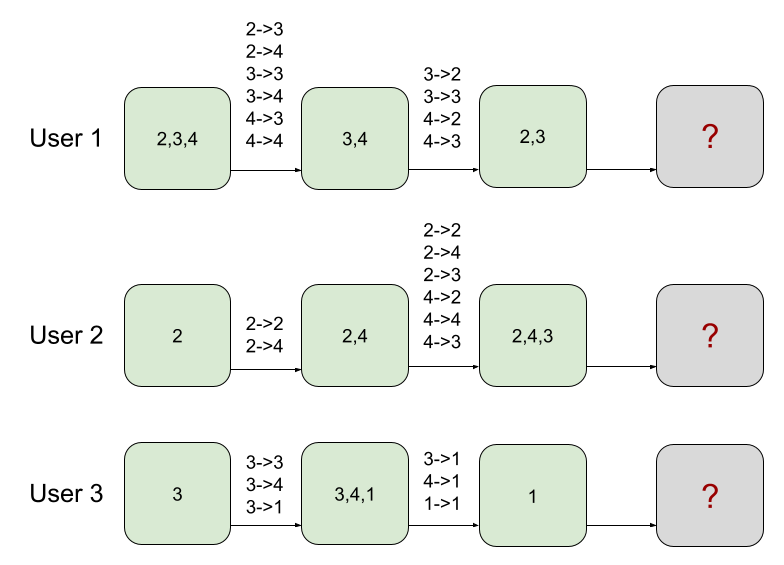
\includegraphics[width=0.8\textwidth]{images/illustrations/markov_chains_recommendations.png}
\caption{The image shows baskets of different users with items. We model the transitions between each item in the old basket to each item in the new basket.}
\label{fig:markov_chains_for_recommendations}
\end{figure}

In Figure~\ref{fig:markov_chains_for_recommendations}, we can see an example of sequences of baskets for three different users. In each basket are items marked with their item number. Going from one basket to another, we can see the transitions from each item in the old basket to each item in the new basket. 

We can now calculate the corresponding Markov chain and transition probabilities as follows:

\begin{equation}
\setlength{\jot}{25pt}
    A_{j,i}=\frac{P(i\in B_t \wedge j\in B_{t-1})}{P(j\in B_{t-1})}=
    \frac{|\{(B_t,B_{t-1}):i\in B_t \wedge j \in B_{t-1}\}|}
    {|\{(B_t,B_{t-1}):j\in B_{t-1}\}|}
    \label{equation:simplified_markov_chain_calc}
\end{equation}

 We will now show how to calculate the Markov chain and the transition matrix for Figure~\ref{fig:markov_chains_for_recommendations} using Equation~\ref{equation:simplified_markov_chain_calc} with a few examples. Illustrated in Figure~\ref{fig:markov_chains_for_recommendations_2} are the results. We recall that baskets are defined as $B^u_t$.

\begin{equation*}
\setlength{\jot}{25pt}
    A_{1,1}=\frac{|(B^3_3,B^3_2)|
}{|(B^3_3,B^3_2)|}=1
\end{equation*}

\begin{equation*}
\setlength{\jot}{25pt}
    A_{2,2}=\frac{|(B^2_2,B^2_1),(B^2_3,B^2_2)|}{|(B^1_2,B^1_1),(B^2_2,B^2_1),(B^2_3,B^2_2)|}=\frac{2}{3}
\end{equation*}

\begin{equation*}
\setlength{\jot}{25pt}
    A_{2,3}=\frac{|(B^1_2,B^1_1),(B^2_3,B^2_2)|}{|(B^1_2,B^1_1),(B^2_2,B^2_1),(B^2_3,B^2_2)|}=\frac{2}{3}
\end{equation*}

\begin{equation*}
\setlength{\jot}{25pt}
    A_{2,4}=\frac{|(B^1_2,B^1_1),(B^2_2,B^2_1),(B^2_3,B^2_2)|}{|(B^1_2,B^1_1),(B^2_2,B^2_1),(B^2_3,B^2_2)|}=1
\end{equation*}

\begin{equation*}
\setlength{\jot}{25pt}
    A_{3,1}=\frac{|(B^3_2,B^3_1),(B^3_3,B^3_2)|}{|(B^1_2,B^1_1),(B^1_3,B^1_2),(B^3_2,B^3_1),(B^3_3,B^3_2)|}=\frac{2}{4}
\end{equation*}


\begin{figure}[htbp]
\centering
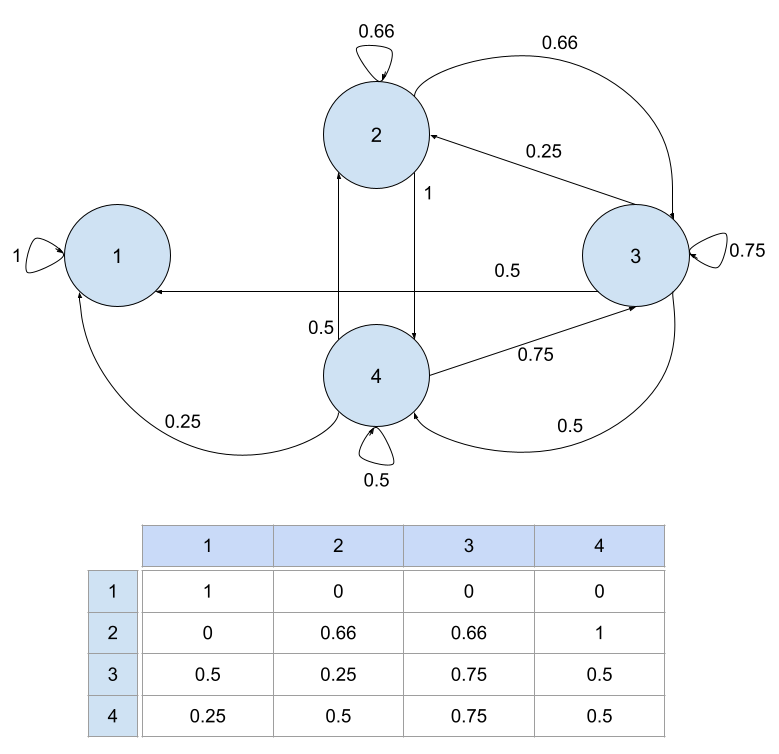
\includegraphics[width=0.8\textwidth]{images/illustrations/markov_chains_recommendations_2.png}
\caption{The image shows the Markov chain as well as the transition probabilities for our example in Figure~\ref{fig:markov_chains_for_recommendations}}
\label{fig:markov_chains_for_recommendations_2}
\end{figure}

Given the Markov chain and transition matrix for our example, we can now make recommendations for the users. We do this by averaging over all transition probabilities as follows:

\begin{equation}
\setlength{\jot}{25pt}
    \hat{P}(i\in B_t |j\in B_{t-1})=\frac{1}{|B_{t-1}|}  \sum_{j\in B_{t-1}} \hat{P}(i\in B_t |j\in B_{t-1})
    \label{equation:simplified_markov_chain_calc_2}
\end{equation}

For our example in Figure~\ref{fig:markov_chains_for_recommendations} we can now calculate the probabilities for the recommendations. For example for User 1:

\begin{equation*}
\setlength{\jot}{25pt}
    \hat{P}(1\in B_t| \{2,3\})=\frac{1}{2}(0+0.5)=0.25
\end{equation*}

\begin{equation*}
\setlength{\jot}{25pt}
    \hat{P}(2\in B_t| \{2,3\})=\frac{1}{2}(0.66+0.25) \approx 0.46
\end{equation*}

\begin{equation*}
\setlength{\jot}{25pt}
    \hat{P}(3\in B_t| \{2,3\})=\frac{1}{2}(0.66+0.75) \approx 0.705
\end{equation*}

\begin{equation*}
\setlength{\jot}{25pt}
    \hat{P}(4\in B_t| \{2,3\})=\frac{1}{2}(1+0.5)=0.75
\end{equation*}

We should not recommend items that the user has already in their basket. Hence, we can discard items 2 and 3. Item 4 has the highest probability therefore we should recommend it to the user.

\section{Shortcomings of Markov Chains}

\begin{figure}[htbp]
\centering
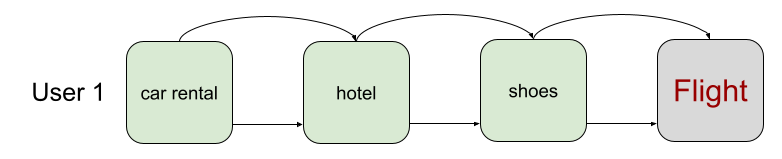
\includegraphics[width=0.8\textwidth]{images/illustrations/markov_chains_shortcomings.png}
\caption{Markov chains only model transitions from one state to another.}
\label{fig:markov_chains_shortcomings}
\end{figure}

\begin{figure}[htbp]
\centering
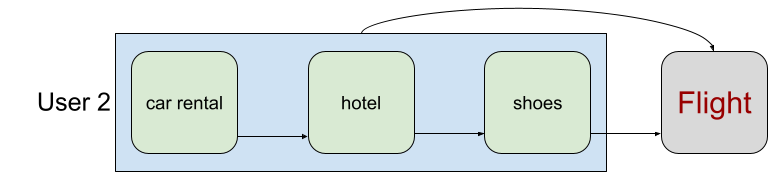
\includegraphics[width=0.8\textwidth]{images/illustrations/markov_chains_shortcomings_2.png}
\caption{We need a more sophisticated model that can look at the whole sequence to make optimal recommendations.}
\label{fig:markov_chains_shortcomings_2}
\end{figure}

While Markov chain models are widely used, they have shortcomings that we want to address~\cite{tang2018personalized}. The Markov chain, models transitions between the sequence only from one item to another. For example, if we take a user who first rents a car, then books a hotel, and then buys shoes. We have illustrated this example in Figure~\ref{fig:markov_chains_shortcomings}. The last item the Markov chain looks at is the shoes. Based on this, it is unlikely that the model will predict that the user will book a flight next. Ideally, we want a model that can factor in the relationship between items of the whole sequence, not just the most recent item. In Figure~\ref{fig:markov_chains_shortcomings_2}, we can see such an example. Fortunately, our BERT model can capture the whole sequence and address these shortcomings.